\documentclass[a4paper,12pt]{article}
\usepackage{amsmath,amssymb}
\usepackage{graphicx}
\usepackage{geometry}
\geometry{margin=2cm}

\begin{document}

\section*{Physik I \hfill Exp. Physik Hausaufgabe}

\subsection*{Aufgabe 1 \hfill Jäger mit Hund}

\[
s(t)=\frac{1}{2}\,\vec a_0\cdot t^2+\vec v_0\,t+s_0
\]

\begin{flushright}
\[
t_0=0h\ (6h)
\]
\[
t_1=2h\ (8h)
\]
\[
\vec v_0=2\cdot \vec v_J
\]
\[
s=10\,\mathrm{km}
\]
\end{flushright}

\subsubsection*{a) $s(t)$ Diagramm}

\begin{center}
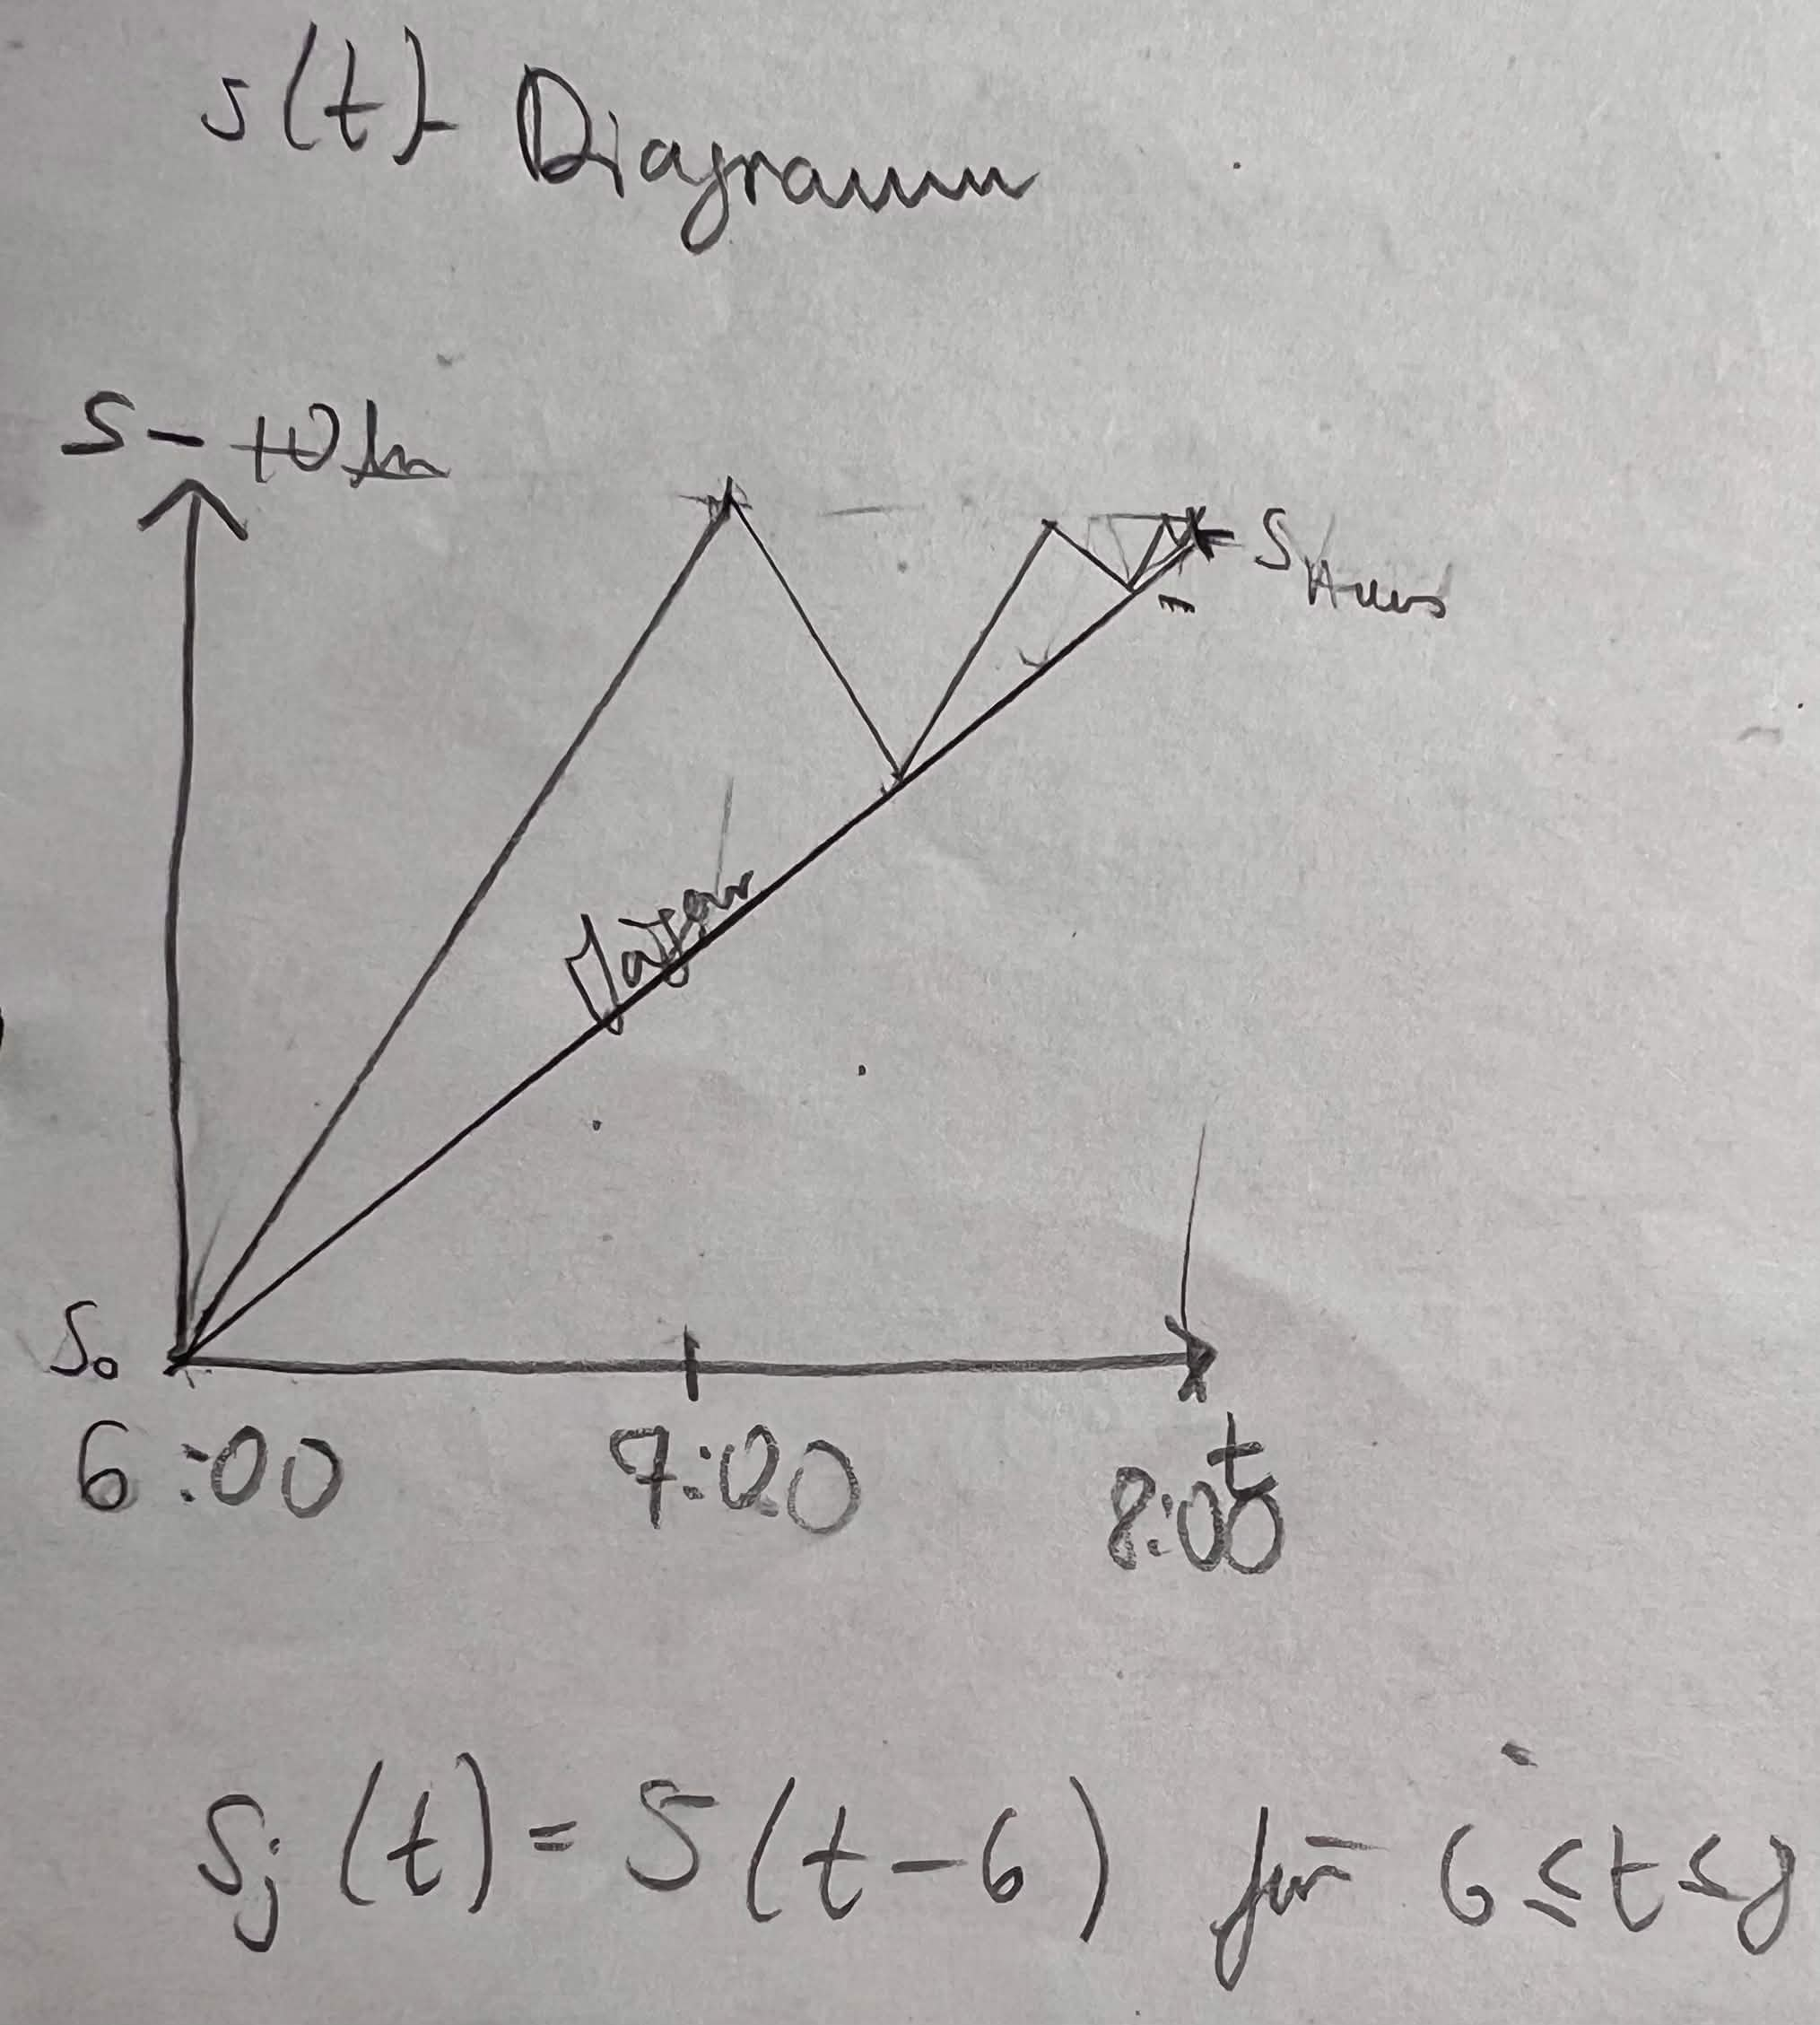
\includegraphics[width=0.5\textwidth]{diagramm1.jpg}
\end{center}

\[
s_J(t)=s(t-6)\qquad \text{für }6<t<8
\]

\subsubsection*{b) Welche Strecke ist der Hund gelaufen}

\[
v_J=\frac{10\,\mathrm{km}}{2h}=5\,\mathrm{km/h}=1{,}38\,\mathrm{m/s}
\]

\[
v_0=2{,}77\,\mathrm{m/s}=10\,\mathrm{km/h}
\]

\[
2h\cdot 10\,\mathrm{km/h}= \boxed{20\,\mathrm{km}}
\]

\vspace{1cm}
\hrule
\vspace{0.7cm}

\subsection*{Aufgabe 2 \hfill Raketenstart}

\[
a=50\,\frac{\mathrm{m}}{\mathrm{s}^2}
\qquad
t=4\,\mathrm{s}
\]

\[
\text{konstant}
\qquad\qquad
\text{senkrecht nach oben }(-9{,}81\,\tfrac{\mathrm{m}}{\mathrm{s}^2})
\]

\subsubsection*{a) \ $\vec v(t)$ bzw. $\vec v(4s)$}

\[
\vec v(t)=\vec a_0\,t+\vec v_0
\]

\[
\vec v(4)=50\,\frac{\mathrm{m}}{\mathrm{s}^2}\cdot 4\,\mathrm{s}+0
\]

\[
v=200\,\frac{\mathrm{m}}{\mathrm{s}}
\]

\subsubsection*{b)}

\[
s_{\max}\ \text{ist bei}\ \vec v(t)=0\ \text{bzw. (ab 4s)}
\]

\[
s(t)=\frac{1}{2}\,\vec a_0\cdot t^2+\vec v_0\,t+s_0
\]

\[
\vec v(t)=\vec a_0\,t+\vec v_0
\]

\begin{center}
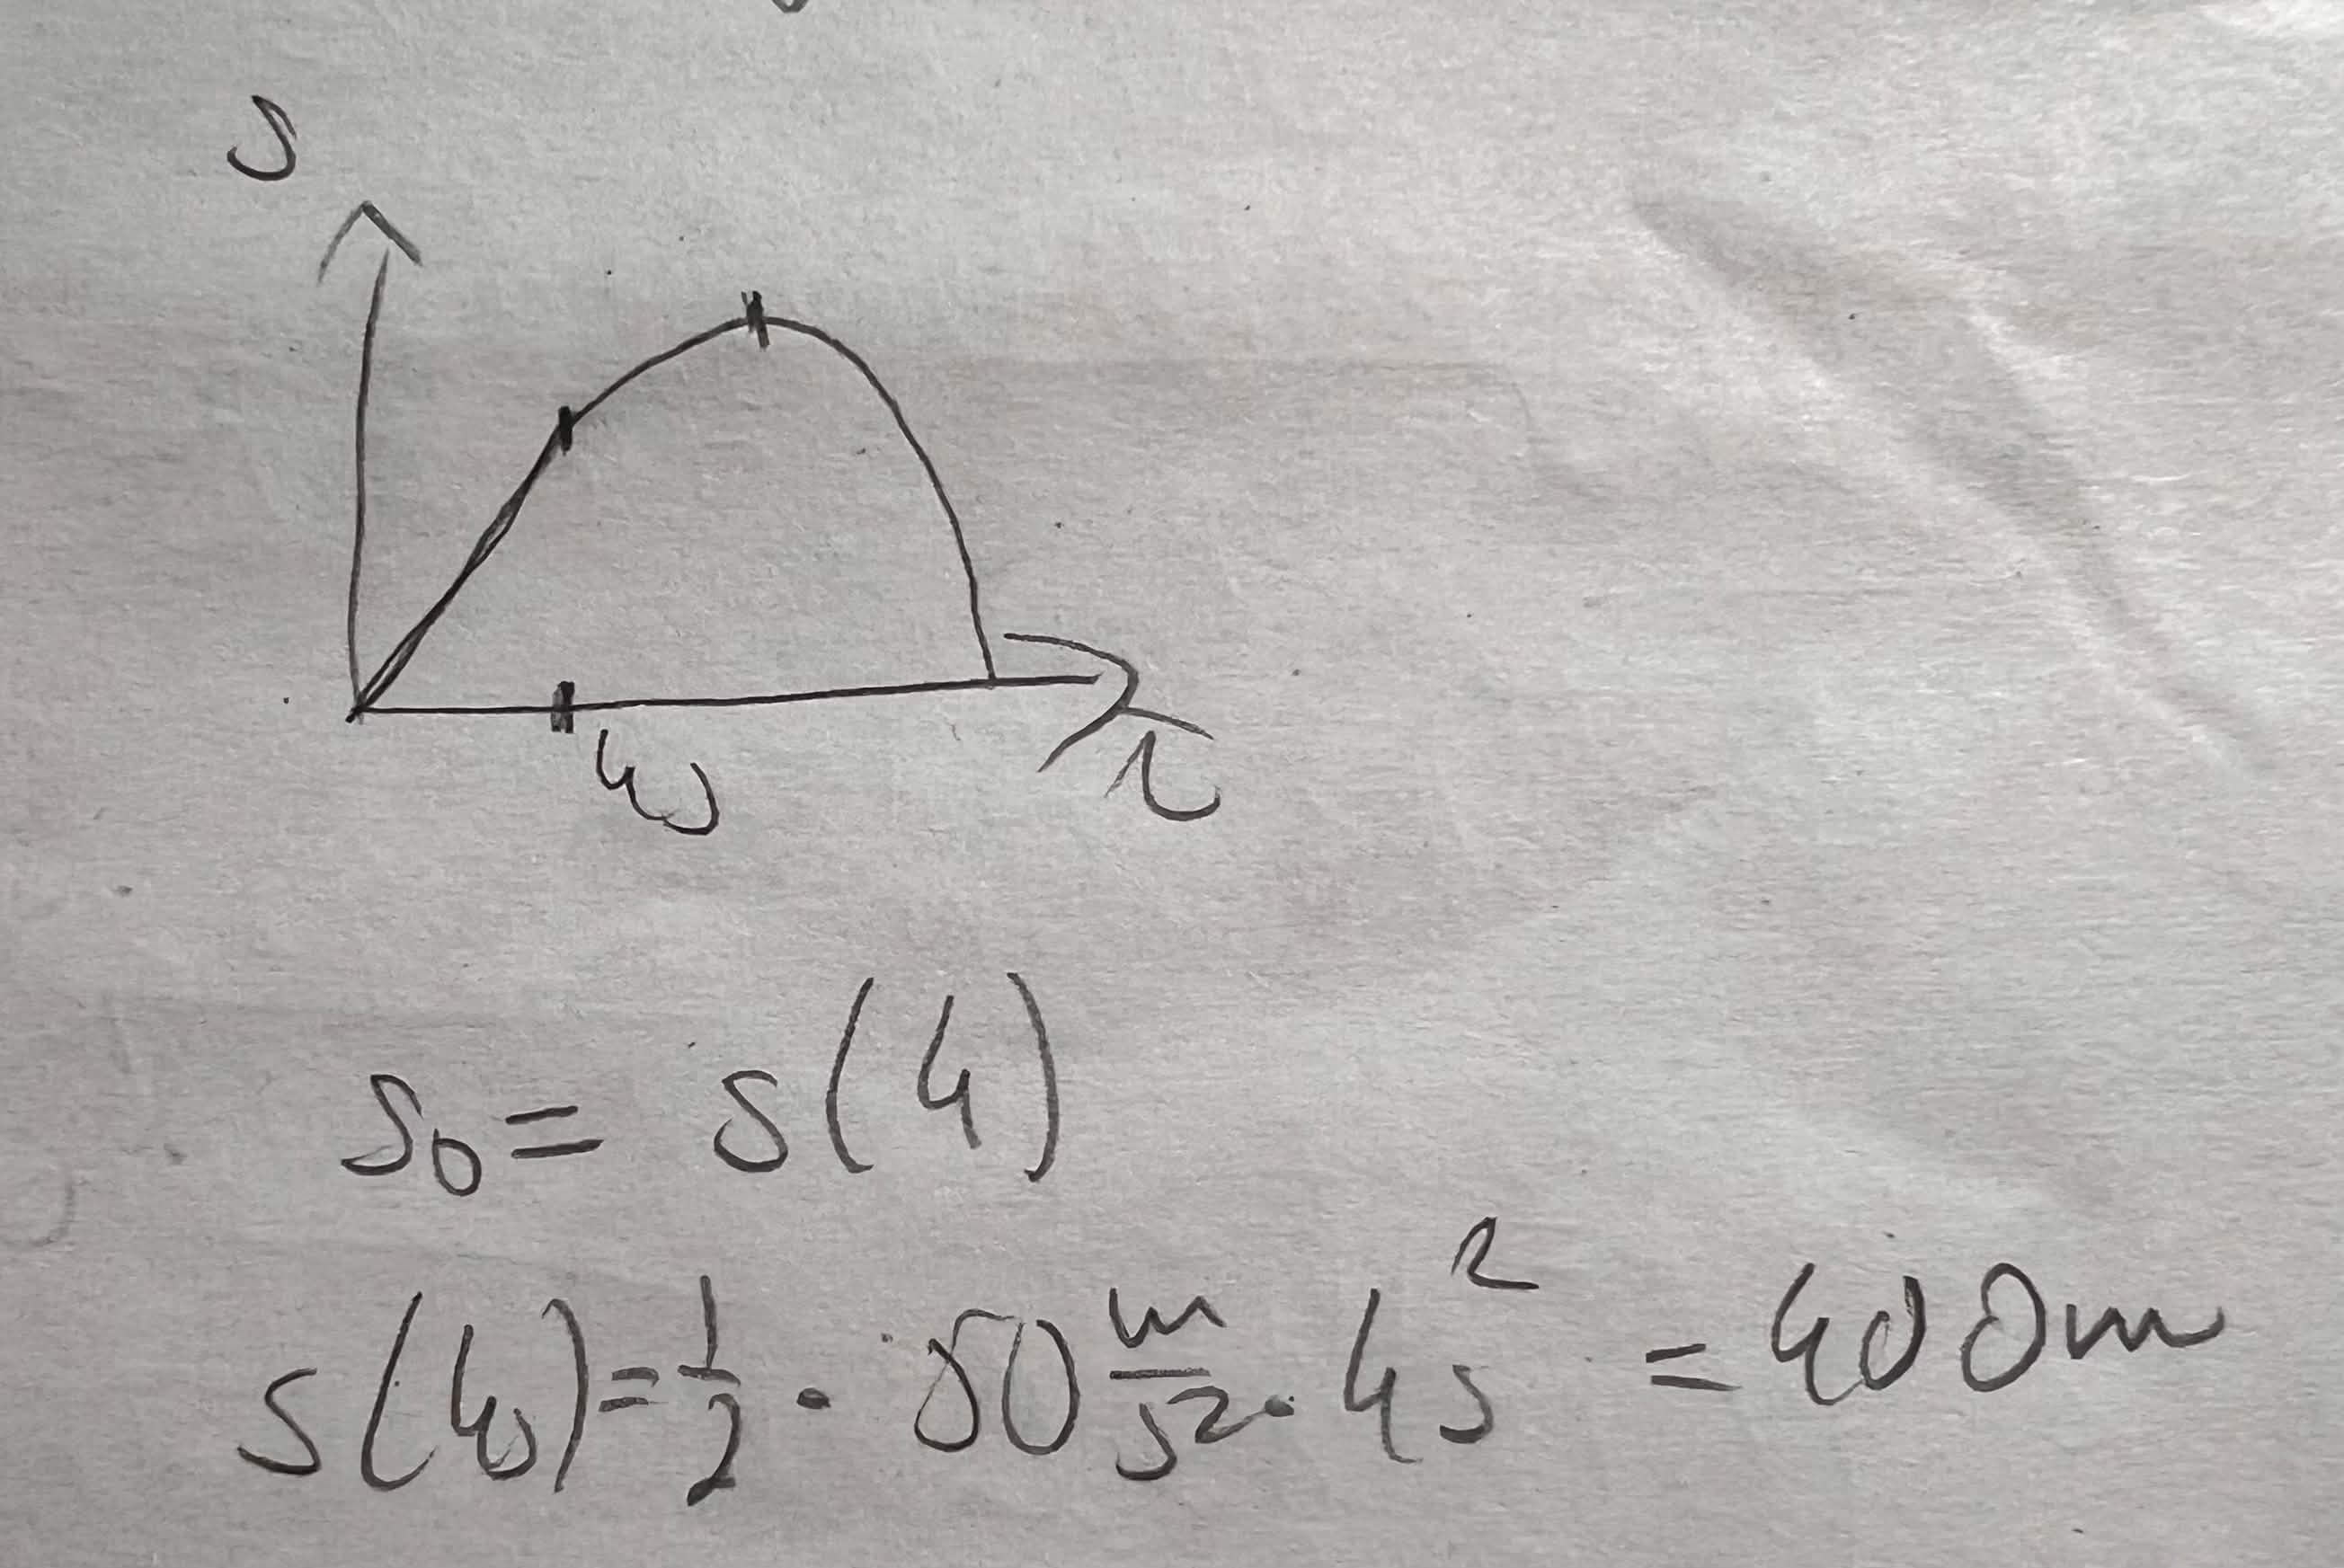
\includegraphics[width=0.4\textwidth]{parabel.jpg}
\end{center}

\[
s_0=s(4)
\]

\[
s(4)=\frac{1}{2}\cdot 50\,\frac{\mathrm{m}}{\mathrm{s}^2}\cdot 4\,\mathrm{s}^2=400\,\mathrm{m}
\]

\[
s(t)=\frac{1}{2}\cdot(-9{,}81)\,t^2+200\,\frac{\mathrm{m}}{\mathrm{s}}\cdot t+400\,\mathrm{m}
\]

\[
\text{Hochpunkt bei }t=20{,}4\,\mathrm{s}
\]

\[
\boxed{2438{,}74\,\mathrm{m}}
\]

\subsubsection*{c) Gesamtdauer}

\[
42{,}7\,\mathrm{s}+4\,\mathrm{s}=46{,}7\,\mathrm{s}
\]

\[
0{,}5\cdot(-9{,}81)t^2+200t+400=0
\]

\[
\text{graphisch bestimmt}
\]

\newpage

\subsection*{Aufgabe 3}

\[
\text{PKW}\qquad l=5\,\mathrm{m},\quad d=40\,\mathrm{m}
\]

\[
\text{LKW}\qquad l=25\,\mathrm{m},\quad v_0=80\,\mathrm{km/h}
\]

\begin{center}
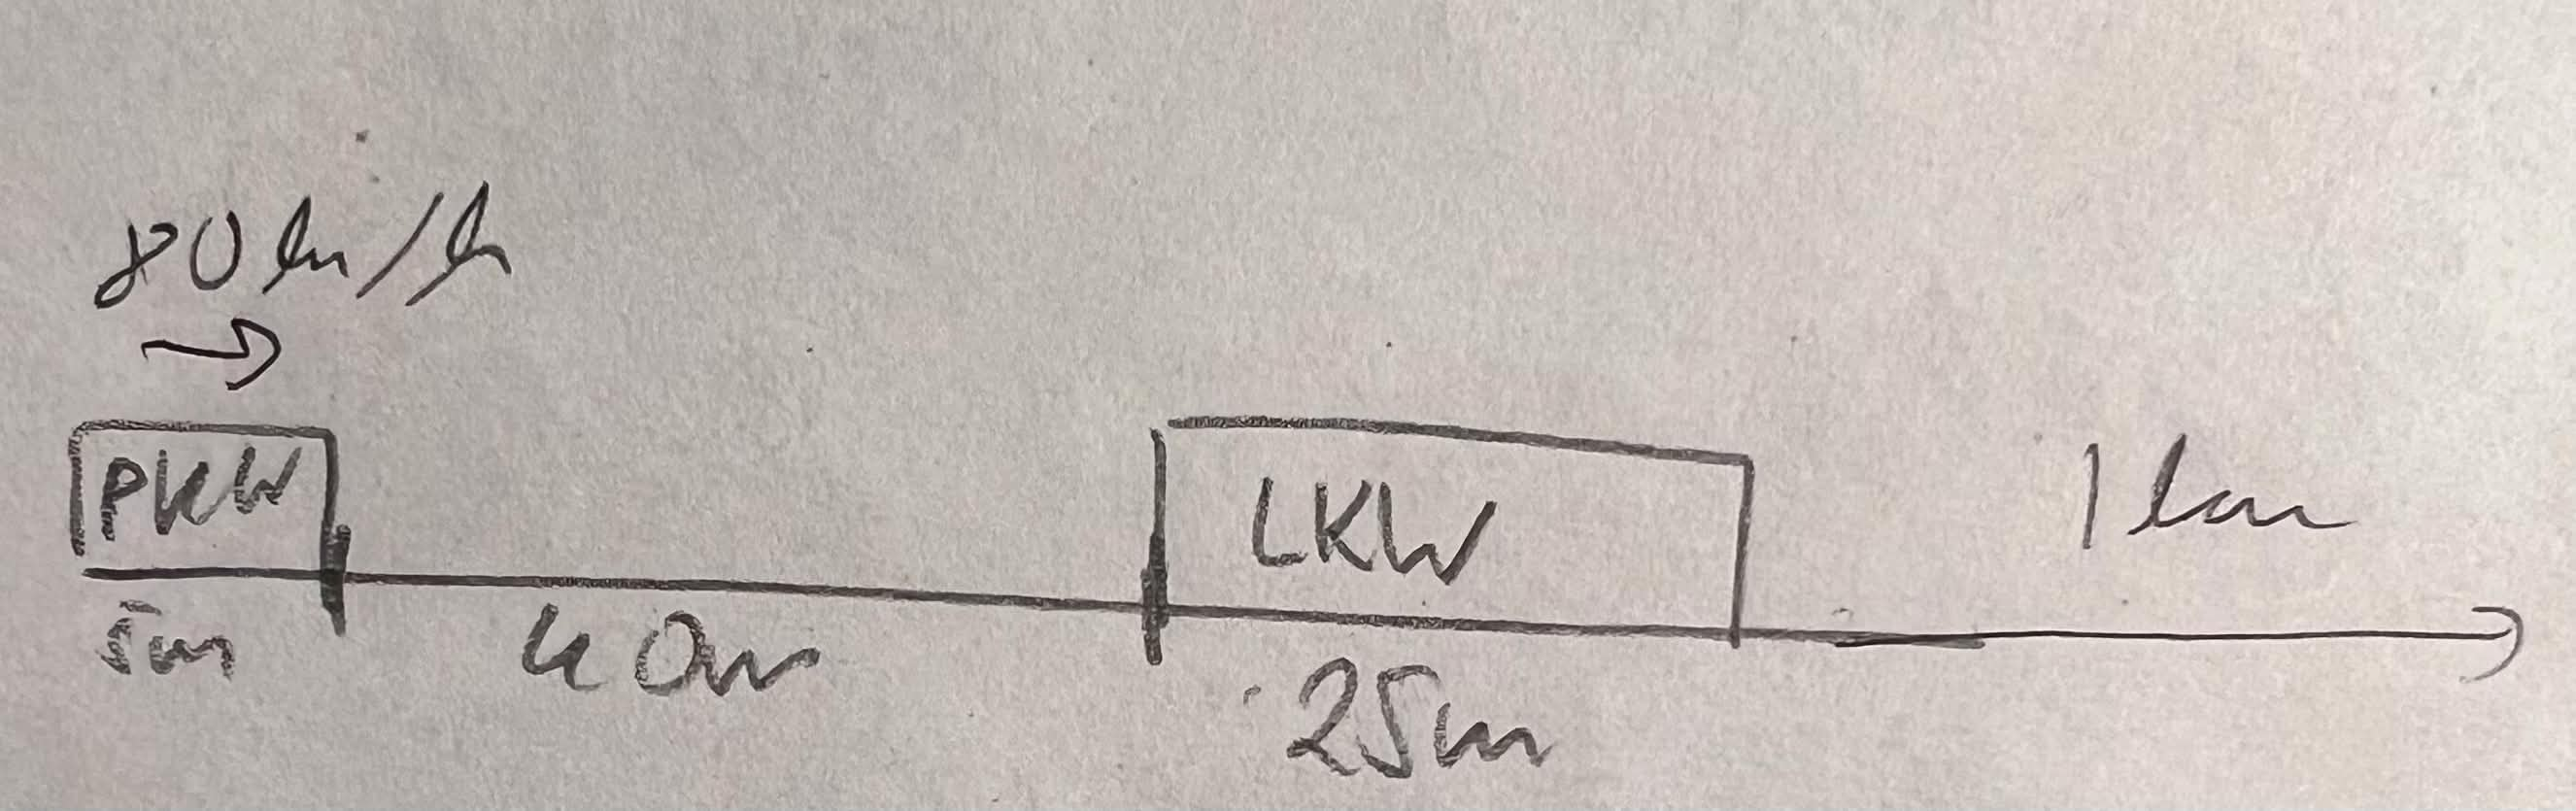
\includegraphics[width=0.8\textwidth]{skizze_pkw_lkw.jpg}
\end{center}

\subsubsection*{a) $s(t)$ Diagramm}

\begin{center}
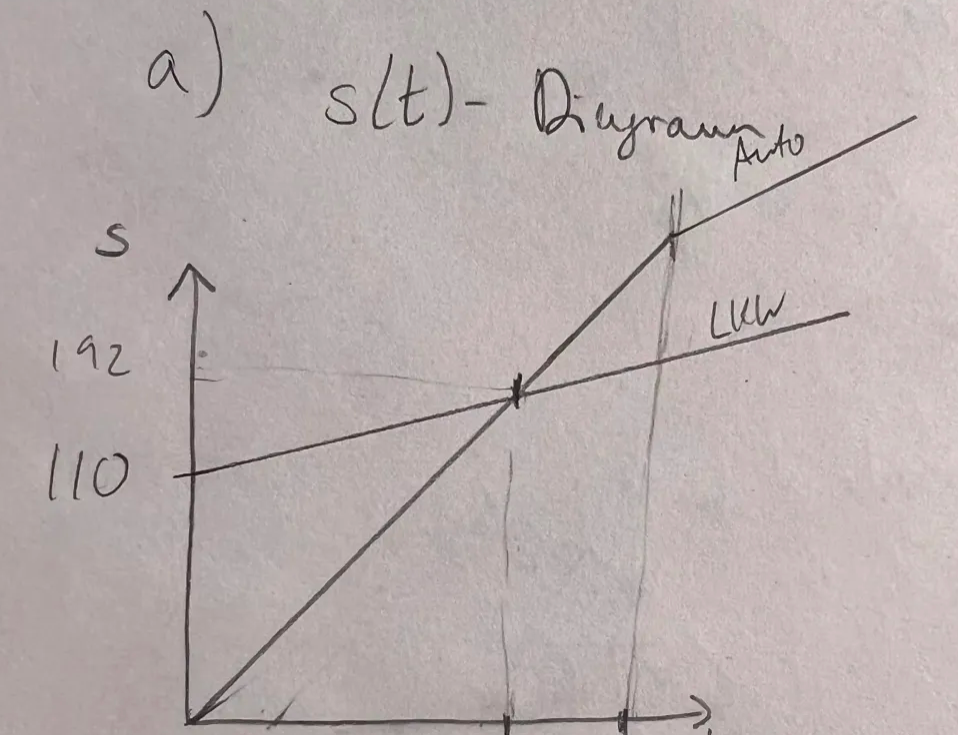
\includegraphics[width=0.7\textwidth]{diagramm2.png}
\end{center}

\[
s_A(t)\ \text{nicht ganz parallel mit }13{,}33\,\mathrm{m}
\]

\[
s_A(t)\Rightarrow \text{wird nach der Strecke gefahren?}
\]

\subsubsection*{b) Wie lange Überholung und dazu benötigte Zeit + 40m Sicherheitsabstand}

\[
s(t)=\frac{1}{2}a_0t^2+v_0t+s_0
\]

\[
\text{Auto beschleunigt zu }100\,\mathrm{km/h}\Rightarrow \text{nur }20\,\mathrm{km/h}\text{ schneller als LKW}
\]

\[
\text{zu überholen: }40\,\mathrm{m}+25\,\mathrm{m}+40\,\mathrm{m}+5\,\mathrm{m}=110\,\mathrm{m}
\]

\[
\Delta v=100-80=20\,\mathrm{km/h}=5{,}55\,\mathrm{m/s}
\]

\[
\vec v_A(t)=a_0t+v_0
\qquad\Rightarrow\qquad
100\,\mathrm{km/h}=1{,}5\,\frac{\mathrm{m}}{\mathrm{s}^2}\cdot t+80\,\mathrm{km/h}
\]

\[
27{,}7\,\frac{\mathrm{m}}{\mathrm{s}}=1{,}5\,\frac{\mathrm{m}}{\mathrm{s}^2}\cdot t+22{,}22\,\frac{\mathrm{m}}{\mathrm{s}}
\]

\[
\Rightarrow t=3{,}7\,\mathrm{s}
\]

\[
s_A(3{,}7\,\mathrm{s})=
\frac{1}{2}\cdot 1{,}5\,\frac{\mathrm{m}}{\mathrm{s}^2}\cdot (3{,}7)^2\,\mathrm{s}^2
+22{,}22\,\frac{\mathrm{m}}{\mathrm{s}}\cdot 3{,}7
=92{,}48\,\mathrm{m}
\]

\[
s_L(3{,}7\,\mathrm{s})=80\,\mathrm{km/h}\cdot 3{,}7\,\mathrm{s}=82{,}22\,\mathrm{m}
\]

\[
92{,}48-82{,}22=10{,}26
\]

\[
110-10{,}26=99{,}74\,\mathrm{m}
\]

\[
t=\frac{99{,}74\,\mathrm{m}}{5{,}55\,\mathrm{m/s}}=17{,}97\,\mathrm{s}
\]

\[
t_{\mathrm{ges}}=3{,}7\,\mathrm{s}+17{,}97\,\mathrm{s}=\boxed{21{,}67}
\]

\[
s_{\mathrm{LKW}}(21{,}67\,\mathrm{s})=
80\,\mathrm{km/h}\cdot 21{,}67\,\mathrm{s}+110\,\mathrm{m}
=\boxed{591{,}56\,\mathrm{m}}
\]

\[
591\,\mathrm{m}<1000\,\mathrm{m}\Rightarrow \text{reicht}
\]

\end{document}